%===================================================================================================
%                                       Capítulo 1 
%===================================================================================================
\chapter{INTRODUÇÃO}\label{cap1}

Este \textit{template} apresenta as regras básicas para a elaboração do trabalho segundo as normas ABNT. Além das regras básicas previstas aqui, solicita-se consultar outros detalhes da norma ABNT sempre que se desejar inserir ou configurar algum elemento não previsto aqui. Ou seja, mesmo que este \textit{template} não preveja as demais regras ABNT, por ser uma visão simplificada, ainda assim elas precisam ser seguidas. 

%---------------------------------------------------------------------------------------------------
\section{Motivação}\label{cap11}

Texto de exemplo, texto de exemplo, texto de exemplo, texto de exemplo, texto de exemplo, texto de exemplo, texto de exemplo, texto de exemplo, texto de exemplo, texto de exemplo, texto de exemplo, texto de exemplo, texto de exemplo, texto de exemplo, texto de exemplo, texto de exemplo, texto de exemplo, texto de exemplo, texto de exemplo, texto de exemplo, texto de exemplo, texto de exemplo, texto de exemplo.

%---------------------------------------------------------------------------------------------------
\section{Objetivos}\label{cap12}

Texto de exemplo, texto de exemplo, texto de exemplo, texto de exemplo, texto de exemplo, texto de exemplo, texto de exemplo, texto de exemplo, texto de exemplo, texto de exemplo, texto de exemplo, texto de exemplo, texto de exemplo, texto de exemplo, texto de exemplo, texto de exemplo, texto de exemplo, texto de exemplo, texto de exemplo, texto de exemplo, texto de exemplo, texto de exemplo, texto de exemplo.Texto de exemplo, texto de exemplo, texto de exemplo, texto de exemplo, texto de exemplo, texto de exemplo, texto de exemplo, texto de exemplo, texto de exemplo, texto de exemplo, texto de exemplo, texto de exemplo, texto de exemplo, texto de exemplo, texto de exemplo, texto de exemplo, texto de exemplo, texto de exemplo, texto de exemplo, texto de exemplo, texto de exemplo, texto de exemplo, texto de exemplo. Texto de exemplo, texto de exemplo, texto de exemplo, texto de exemplo, texto de exemplo, texto de exemplo, texto de exemplo, texto de exemplo, texto de exemplo, texto de exemplo, texto de exemplo, texto de exemplo, texto de exemplo, texto de exemplo, texto de exemplo, texto de exemplo, texto de exemplo, texto de exemplo, texto de exemplo, texto de exemplo, texto de exemplo, texto de exemplo, texto de exemplo.

\section{Justificativa}\label{cap13}


\begin{table}[htbp]
	\centering
	\caption{Exemplo de título de tabela}
	\begin{tabular}{p{1in} p{1in} p{1in} p{1in} } \hline
		
		Cabeçalho 1	& Cabeçalho 2	& Cabeçalho 3	& Cabeçalho 4 \\ \hline
		Texto	& número & número	& número \\ 
		Texto	& número & número	& número \\ 
		Texto	& número & número	& número \\ 
		Texto	& número & número	& número \\ 
		Texto	& número & número	& número \\ \hline
		
	\end{tabular}
	\label{tab:ExemploDeTabela1}
\end{table}


Atenção ao fazer citações a referências para garantir o uso da forma correta, considerando os seguintes exemplos:
\begin{itemize}
	\item Se desejar que uma citação a uma referência apareça no final da frase, use com o comando ``citep''. Exemplo: ``Tal coisa é muito melhor do que aquela outra coisa \citep{Modest2013, Modest2016}''
	\item Se desejar que uma citação a uma referência apareça no meio da frase, como parte da própria frase, use o comando ``citet''. Exemplo: ``De acordo com \citet{Modest2013}, tal coisa é muito melhor do que aquela outra coisa.''
	\item \textbf{Atenção} - nunca usar o comando ``citep'' para citações a referências que aparecem no meio da frase, como parte da própria frase. Exemplo: ``De acordo com \citep{Modest1991}, tal coisa é muito melhor do que aquela outra coisa.''
\end{itemize}

\begin{figure}[!h] 
	\centering
	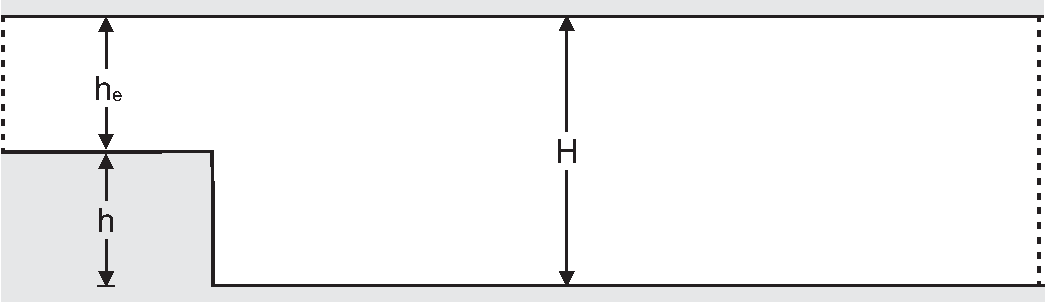
\includegraphics[width=1\textwidth]{./cap1/figs/Canal.pdf}
	\caption{Exemplo de uma figura simples.}
	\label{fig:F2}
\end{figure}

\begin{figure}[!t] 
	\centering
	\subfigure[Solução A]{
		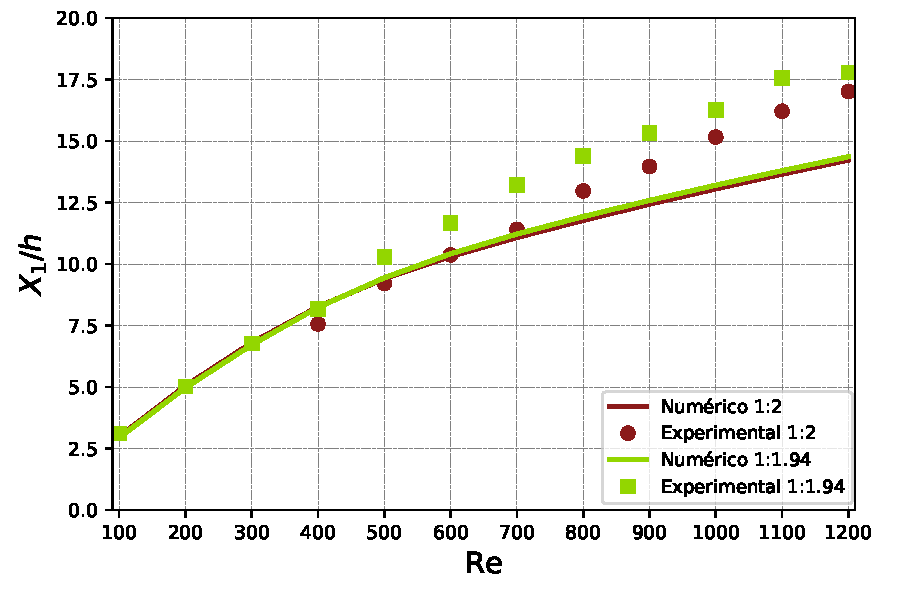
\includegraphics[width=0.45\textwidth]{./cap1/figs/CLAX1.pdf}
		\label{F1A}
	}\hfil
	\subfigure[Solução B]{
		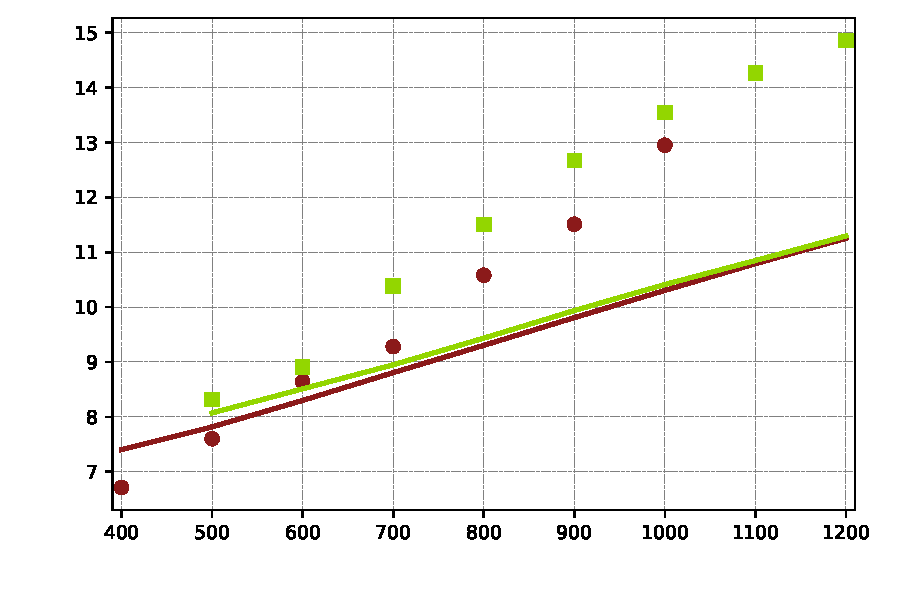
\includegraphics[width=0.45\textwidth]{./cap1/figs/CLAX2.pdf}
		\label{F1B}
	}
	\subfigure[Solução C]{
		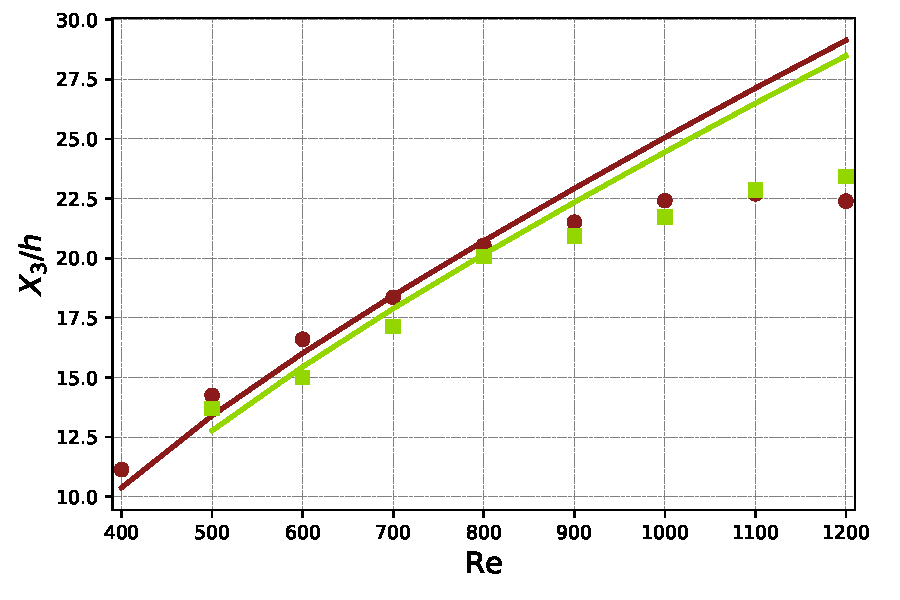
\includegraphics[width=0.45\textwidth]{./cap1/figs/CLAX3.pdf}
		\label{F1C}
	}\hfil
	\subfigure[Solução D]{
		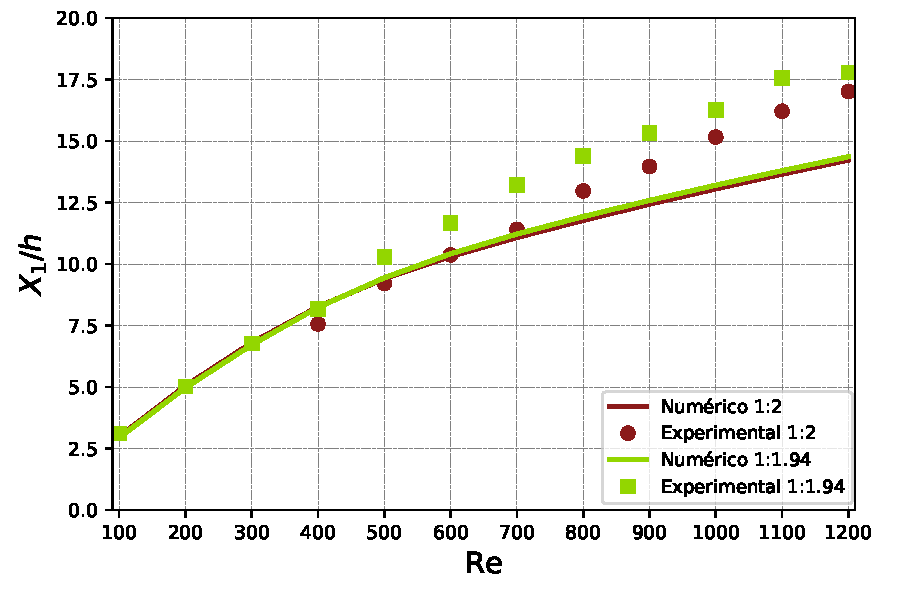
\includegraphics[width=0.45\textwidth]{./cap1/figs/CLAX1.pdf}
		\label{F1D}
	}
	\caption{Exemplo de quatro figuras agrupadas.}
	\label{fig:F1}
\end{figure}



\begin{table}[H]
	\centering
	\caption{Exemplo de Cronograma.}
	\begin{center}
		\begin{tabular}{*{16}{|c} |c|}\hline
			\multirow{2}{*}{Etapas} & \multicolumn{4}{|c|}{2019}& \multicolumn{4}{|c|}{2020}& \multicolumn{4}{|c|}{2021}& \multicolumn{4}{|c|}{2022}\\ \cline{2-17}
			& $1^o$  & $2^o$ & $3^o$ & $4^o$ & $1^o$  & $2^o$  & $3^o$ & $4^o$ & $1^o$  & $2^o$ & $3^o$ & $4^o$ & $1^o$  & $2^o$  & $3^o$ & $4^o$ \\\hline
			A & x & x & x & x & x & x & x & x & x & x & x & x & x & x & x & x  \\\hline
			B & x & x & x & x &   &   &   &   &   &   &   &   &   &   &   &   \\\hline
			C &   &   & x & x & x &   &   &   &   &   &   &   &   &   &   &   \\\hline
			D &   &   &   &   & x & x & x & x &   &   &   &   &   &   &   &   \\\hline
			E &   &   &   &   &   &   & x & x & x & x &   &   &   &   &   &   \\\hline
			F &   &   &   &   &   &   &   & x & x & x & x & x &   &   &   &   \\\hline
			G &   &   &   &   &   &   &   &   & x & x & x & x &   &   &   &   \\\hline
			H &   &   &   &   &   &   &   &   &   & x & x & x & x &   &   &   \\\hline
			I &   &   &   &   &   &   &   &   &   &   &   & x & x & x & x & x  \\\hline
			J &   &   &   &   &   &   &   &   &   &   &   & x & x & x & x & x \\\hline
			K &   &   &   &   &   & x &   & x &   & x &   & x &   & x &   & x  \\\hline
			L &   &   &   &   &   &   &   &   &   & x & x & x & x & x & x & x  \\\hline
		\end{tabular}
		\label{tab:crono}
	\end{center}
\end{table}